% command to make sure colorboxes don't create whitespace between code lines
\fboxsep=.6pt

% default settings for listings
\lstset{style=python}

\title[Programmieren]{Programmieren}

\subtitle{\emoji{woman-technologist} Logische Ausdrücke}

\author[Wendl, Cyril] % (optional)
{Cyril Wendl \inst{1}}

\institute[KZN] % (optional)
{
  \inst{1}%
  Fachschaft Informatik\\
  Kantonsschule im Lee
}

\date[\today] % (optional)

\logo{\includegraphics[width=.8cm]{\thelogo}}

\titlegraphic{\includegraphics[width=\textwidth]{"GrundlagenInfo/06_Daten/Figures/title-emojis"}}

\frame{\titlepage}



\begin{frame}[fragile]{Verzweigungen: allgegenwärtig}
    \begin{itemize}[<+->]
        \item Promotionsentscheid (Notendurchschnitt)
              \only<1>{\begin{figure}[H]
                      \centering
                      \begin{tikzpicture}[transform shape, scale=.7, on grid, ->]
                          \tikzstyle{every node}=[font=\small]
                          % grid to easier see that the node centers line up while developing plot
                          %\draw [help lines] (-5,-9) grid (9,1);
                          \node (start) [code] {\lstinline|note_schnitt = 3.6|};
                          \node (dec1) [decision, below=2.5cm of start] {\lstinline|note_schnitt >= 3.75|};
                          \node (printif) [code, below left=1.5cm and 4cm of dec1] {\lstinline|print("Semester bestanden")|};
                          \node (printelse) [code, below right=1.5cm and 4cm of dec1] {\lstinline|print("Semester nicht bestanden")|};
                          \node (end) [circle,draw=black, fill=black, below=3cm of dec1] {};

                          \draw (start) -- (dec1);
                          \draw (dec1) -| node[anchor=top, above=.1cm] {\lstinline|True|} (printif);
                          \draw (dec1) -| node[anchor=top, above=.1cm] {\lstinline|False|} (printelse);
                          \draw (printif) |- (end);
                          \draw (printelse) |- (end);

                      \end{tikzpicture}
                  \end{figure}}
        \item Wie gehe ich zur Schule?
              \only<2>{\begin{figure}[H]
                      \centering
                      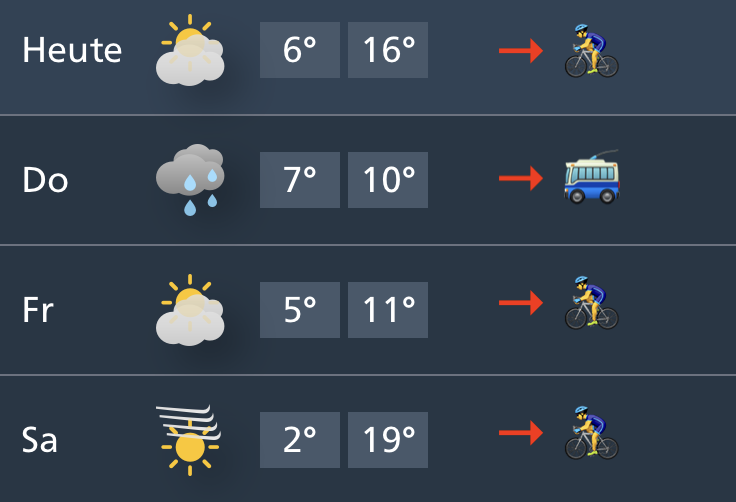
\includegraphics[width=0.7\linewidth]{GrundlagenInfo/00_Programmieren/Figures/if-elif-else-weather}
                  \end{figure}
                  $\rightarrow$ \textit{und wenn ich gesund bin / mich bewegen kann}}
        \item Medizinische Entscheide
              \only<3>{\begin{figure}[H]
                      \centering
                      
\includegraphics[width=0.7\linewidth]{GrundlagenInfo/00_Programmieren/Figures/if-elif-else-cancer}
                  \end{figure}
                  $\rightarrow$ \textit{Und wenn die Fachärzte dies bestätigen}}
        \item Etc.
    \end{itemize}
\end{frame}


\begin{frame}[fragile]{Negation von Aussagen}
	\begin{table}
	\begin{tabular}{p{5cm}|p{5cm}}
	\textbf{Aussage} & \textbf{Negation} \\\midrule\midrule
	\visible<+->{``Das Mädchen heisst Elin''}& \visible<+->{``Das Mädchen heisst nicht Elin''}\\\midrule
	\visible<+->{``Niemand in dieser Klasse ist volljährig''}& \visible<+->{``Mindestens eine Person in dieser Klasse ist volljährig''}\\\midrule
	\visible<+->{$x > 2$} & \visible<+->{$x \leq 2$}
	\end{tabular}
	\end{table}
	\only<7->{
	    \begin{figure}[H]
	    \centering
	    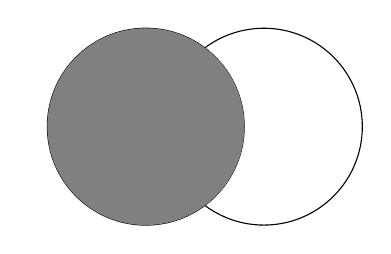
\begin{tikzpicture}
	      \tikzset{circle node/.style={circle,draw=black, fill=none, minimum size=25mm, inner sep=0pt}}
	      \node[circle node] (left) at (0,0) {};
	      \node[circle node] (right) at (1.5,0) {};
	      \begin{scope}
	        \clip (-1.5,-1.25) rectangle (1.25,1.25);
	        \fill[gray] (0,0) circle (1.25cm);
	      \end{scope}
	      \begin{scope}
	        \clip (0,0) circle (1.25cm);
	        \fill[gray] (1.5,0) circle (1.25cm);
	      \end{scope}
	    \end{tikzpicture}
	    \end{figure}}
\end{frame}

\begin{frame}[fragile]{Negation von Aussagen}
\href{https://youtu.be/3UEWiZCT4oM?feature=shared}{Link: Mani Matter}
\end{frame}


\begin{frame}{Auftrag (10')}
\begin{itemize}
    \item \aufgabebox{Aufgaben 4.15 - 4.18}
\end{itemize}

\end{frame}


\begin{frame}[fragile]{Negation von Aussagen in Python: \lstinline|not|}
\begin{columns}
\begin{column}{.25\textwidth}
\begin{lstlisting}
if x == 0:
	...
\end{lstlisting}
\end{column}
\begin{column}{.15\textwidth}
$\underrightarrow{\text{Negation:}}$
\end{column}
\begin{column}{.5\textwidth}
Entweder:
\begin{lstlisting}
if x != 0:
	...
\end{lstlisting}

Oder:
\begin{lstlisting}
if not x == 0:
	...
\end{lstlisting}
\end{column}
\end{columns}
\end{frame}

\begin{frame}[fragile]{Modulo: Rest von Ganzzahldivision}
\begin{itemize}[<+->]
\item 12/5 = ``2 komma etwas'' (genauer gesagt 2.4)
\item wie viel ist nicht ganz durch 5 teilbar?
\item 2 
\item In Python: \lstinline|12 % 5|

\item \lstinline|x % 5 == 0| zeigt uns also an, ob eine \lstinline|x| durch 5 teilbar ist
\item Wie finden wir heraus, ob \lstinline|x| eine gerade Zahl ist?
\item \lstinline|x % 2 == 0|
\end{itemize}
\end{frame}

\begin{frame}[fragile]{Modulo: Beispiel}
\begin{table}
	\begin{tabular}{r|l}
	\textbf{Code} & \textbf{Resultat} \\\midrule\midrule
	\lstinline|1 % 3|& \lstinline|?|\\\midrule
	\lstinline|2 % 3|& \lstinline|?|\\\midrule
	\lstinline|3 % 3|& \lstinline|?|\\\midrule
	\lstinline|4 % 3|& \lstinline|?|\\\midrule
	\lstinline|5 % 3|& \lstinline|?|\\\midrule
	\lstinline|6 % 3|& \lstinline|?|\\\midrule
	\lstinline|...|& \lstinline|...|
	\end{tabular}
\end{table}
\end{frame}
\begin{frame}[fragile]{Modulo: Beispiel}
\begin{table}
	\begin{tabular}{r|l}
	\textbf{Code} & \textbf{Resultat} \\\midrule\midrule
	\lstinline|1 % 3|& \lstinline|1|\\\midrule
	\lstinline|2 % 3|& \lstinline|2|\\\midrule
	\lstinline|3 % 3|& \lstinline|0|\\\midrule
	\lstinline|4 % 3|& \lstinline|1|\\\midrule
	\lstinline|5 % 3|& \lstinline|2|\\\midrule
	\lstinline|6 % 3|& \lstinline|0|\\\midrule
	\lstinline|...|& \lstinline|...|
	\end{tabular}
\end{table}

\begin{itemize}[<+->]
\item Wie finden wir heraus, welche Zahlen \lstinline|x| durch 3 teilbar sind?
\item \lstinline|x % 3 == 0|
\end{itemize}
\end{frame}

\begin{frame}[fragile]{Mehrere Bedingungen zusammenfassen}
\begin{columns}
\begin{column}{.4\textwidth}
\begin{lstlisting}[escapechar=!,basicstyle=\tiny\ttfamily]
antwort = input("Nenne einen Kanton, in dem man Italienisch spricht")

if antwort == "Tessin":         !\tikzmark{fromStart}!
    print("Richtig")

elif antwort == "Graubünden": 
    print("Richtig")            !\tikzmark{fromEnd}!

else:
    print("Falsch")
\end{lstlisting}
\end{column}
\begin{column}{.6\textwidth}
\begin{lstlisting}[escapechar=!,basicstyle=\tiny\ttfamily]
antwort = input("Nenne einen Kanton, in dem man Italienisch spricht")

!\tikzmark{toStart}!if antwort == "Tessin" or antwort == "Graubünden":
!\tikzmark{toEnd}!    print("Richtig")

else:
    print("Falsch")
\end{lstlisting}
\end{column}
\end{columns}

% annotate listings
\begin{tikzpicture}[overlay, remember picture,
    every edge/.append style = { ->, thick, >=stealth, red!70},
    every node/.style={draw=red!50,fill=red!50!white,text=black,rounded corners}]
	\only<2->{
	\drawBrace{0em}{fromStart}{fromEnd}{}{.5}{}{}
	\drawBrace{-.5em}{toStart}{toEnd}{}{.5}{mirror}{}
	 % arrow pointing from one code to other
  \draw[->, style={thick, >=stealth, red!70}] (fromStartfromEnd-coord-arrow) to (toStarttoEnd-coord-arrow);
		}
\end{tikzpicture}
\only<3>{
Wie könnten die beiden Bedingungen im ersten \lstinline|if| negiert werden?}
\end{frame}

\begin{frame}[fragile]{Zusammenfassung}
\begin{itemize}
	\item Mit einem \lstinline|not| kann ein logischer Ausdruck \textit{negiert} werden
	\item Mit den Befehlen \lstinline|and| sowie \lstinline|or| können logische Ausdrücke miteinander \textit{verknüpft} werden.
\end{itemize}
\end{frame}

\begin{frame}{Auftrag}
	% TODO update with Skript
\begin{itemize}
    \item Lesen Sie Beispiel 4.5
    \item \aufgabebox{Aufgaben 4.22 - 4.26}
    \item \abgabebox{Aufgaben 4.19, 4.25 (Moodle)}
\end{itemize}
\end{frame}


% \begin{frame}[fragile]{Mehrere Bedingungen zusammenfassen}{Negation mehrere Bedingunge}

% 	\begin{lstlisting}[escapechar=!]
% 	antwort = input("Nenne einen Kanton, in dem man Italienisch spricht")
	
% 	if !\colorbox{CarnationPink}{not (}!antwort == "Tessin" or antwort == "Graubünden"!\colorbox{CarnationPink}{)}!:
% 		print("Falsch")
% 	else:
% 		print("Richtig")
% 	\end{lstlisting}
	
% 	oder:
	
% 	\begin{lstlisting}[escapechar=!]
% 	antwort = input("Nenne einen Kanton, in dem man Italienisch spricht")
	
% 	if not antwort == "Tessin" !\colorbox{CarnationPink}{and}! not antwort == "Graubünden":
% 		print("Falsch")
% 	else:
% 		print("Richtig")
% 	\end{lstlisting}
% 	\end{frame}